\documentclass{article}

\usepackage[margin=0.5in]{geometry}
\usepackage{multicol}
\usepackage{graphicx}
\usepackage{tkz-euclide}
\usepackage{amsmath}

\title{Problem-Solving Set B}
\author{}
\date{}

\begin{document}
\maketitle
\noindent Problems should be solved without a calculator unless otherwise specified.
Remember to explain how you solved a problem.
\begin{multicols*}{2}
    \begin{enumerate}
        \item A bar graph shows the number of hamburgers sold by a fast food chain each season.
            However, the bar indicating the number sold during the winter covered by a smudge.
            If exactly $25\%$ of the chain's hamburgers are sold in the fall, how many million hamburgers are sold in the winter?
            \begin{center}
                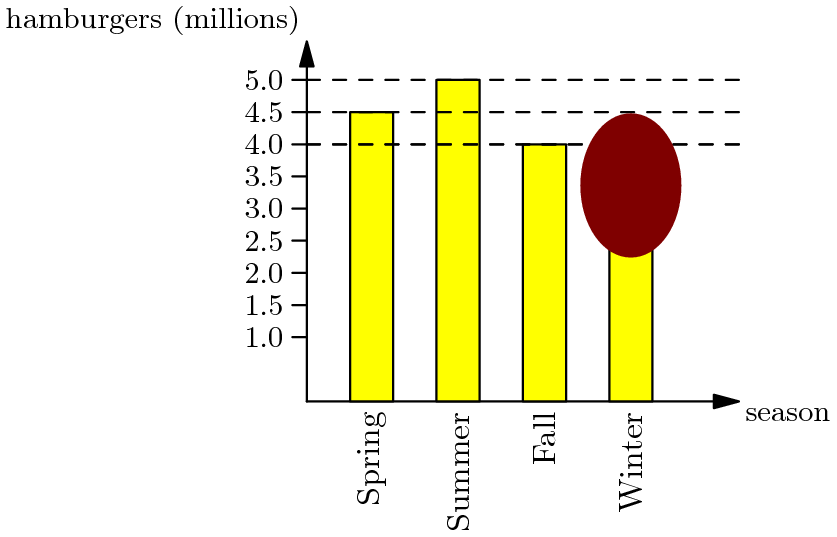
\includegraphics[scale=0.2]{5-2_bar_graph.png}
            \end{center}
            \vspace{3cm}
        \item Suppose one of the eight lettered identical squares included with the four squares in the T-shaped figure outlined.
            How many of the resulting figures can be folded into a topless cubical box.
            \begin{center}
                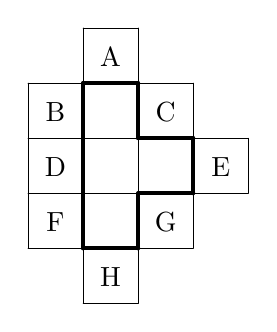
\begin{tikzpicture}[scale=0.7]
                    \foreach \xcoord\ycoord\name in {0/1/A1, 0/4/A2, 1/0/B1, 1/5/B2, 2/0/C1, 2/5/C2, 3/1/D1, 3/4/D2, 4/2/E1, 4/3/E2, 0/2/F1, 0/3/F2}
                    {
                        \tkzDefPoint(\xcoord,\ycoord){\name}
                    }
                        
                    \tkzDrawSegments(A1,A2 B1,B2 C1,C2 D1,D2 E1,E2)
                    \tkzDrawSegments(B2,C2 A2,D2 F2,E2 F1,E1 A1,D1 B1,C1)

                    \foreach \x\y\d\z\name in {B1/B2/A2/D2/I1, C1/C2/A2/D2/I2, C1/C2/F2/E2/I3, D1/D2/F2/E2/I4, D1/D2/F1/E1/I5, C1/C2/F1/E1/I6, C1/C2/A1/D1/I7, B1/B2/A1/D1/I8, B1/B2/F2/E2/J2, B1/B2/F1/E1/J1}
                    {
                        \tkzInterLL(\x,\y)(\d,\z)
                        \tkzGetPoint{\name}
                    }
                    \tkzDrawSegments[line width = 0.5mm](I1,I2 I2,I3 I3,I4 I4,I5 I5,I6 I6,I7 I7,I8 I8,I1)
                    \foreach \x\y\name in {B2/C2/A, A2/I1/B, I2/D2/C, F2/J2/D, I4/E2/E, F1/J1/F, I6/I5/G, I8/I7/H}
                    {
                        \tkzLabelSegment[below, yshift=-3.5](\x,\y){\name}
                    }
                \end{tikzpicture}
            \end{center}
            \vspace{3cm}
        \item If $A$ and $B$ are nonzero digits, then the number of digits (not necessarily different) in the sum of three whole numbers is:
            $$\begin{tabular}{ccccc}
                9 & 8 & 7 & 6 \\
                & A & 3 & 2 \\
                & B & 1 & \\
                \hline
            \end{tabular}$$
            How many digits are in the answer?
            \vspace{3cm}
        \item $ABCD$ is a rectangle, $D$ is the center of the circle, and $B$ is on the circle.
            If $AD = 4$ and $CD = 3$, then the area of the shaded region is between which two integers?
            \begin{center}
                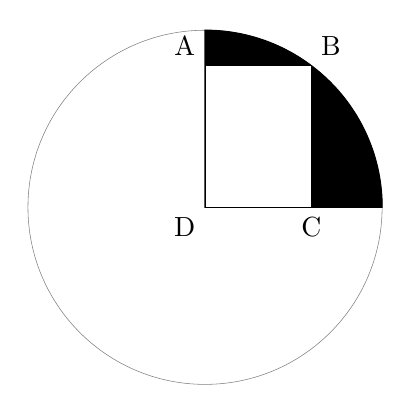
\begin{tikzpicture}[scale=0.45]
                    \tkzDefPoint(0,0){D}
                    \tkzDefPoint(0,4){A}
                    \tkzDefPoint(3,4){B}
                    \tkzDefPoint(3,0){C}
                    \tkzDefPoint(0,5){E}
                    \tkzDefPoint(5,0){F}

                    \tkzDrawCircle(D,B)
                    \tkzDrawSector[fill=black](D,F)(E)

                    \tkzDrawPolygon[fill=white](D,A,B,C)
                    \tkzLabelPoint[above left](A){A}
                    \tkzLabelPoint[above right](B){B}
                    \tkzLabelPoint(C){C}
                    \tkzLabelPoint[below left](D){D}
                \end{tikzpicture}
            \end{center}
            \vspace{3cm}
        \item A palindrome is a whole number that reads the same forwards and backwards.
            If one neglects the colon, certain times displayed on a digital watch are palindromes.
            Three examples are $1\colon 01$, $4\colon 44$, and $12\colon 21$.
            How many times during a $12$-hour period will be palindromes?
            \vspace{3cm}
    \end{enumerate}
\end{multicols*}
\end{document}
